\documentclass[a4paper,12pt]{extarticle}
\usepackage[table,xcdraw]{xcolor}
\usepackage{pgfplots}
\usepackage[unicode, pdftex]{hyperref}
\usepackage[T2A]{fontenc}
\usepackage[utf8]{inputenc}
\usepackage[english,russian]{babel}
\usepackage{amsmath,amsfonts,amsthm, mathtools}
\usepackage{amssymb}
\usepackage{graphicx}
\graphicspath{{images/}}
\usepackage{wrapfig}
\usepackage{floatrow}
\usepackage{setspace}
\usepackage[headings]{fancyhdr}
\usepackage[margin=10pt,font={small,stretch=0,9},labelfont=bf,labelsep=period,
justification=centerlast]{caption}
\usepackage{array,tabularx,tabulary,booktabs}
\RequirePackage{multirow}
\RequirePackage{multicol}
\RequirePackage{longtable}
\usepackage{indentfirst}
\usepackage{hyperref}
\usepackage{icomma}
\newcommand*{\hm}[1]{#1\nobreak\discretionary{}
	{\hbox{$\mathsurround=0pt #1$}}{}}
\usepackage{soulutf8} 
\usepackage{etoolbox} 
\usepackage{geometry}
\geometry{top=20mm}
\geometry{bottom=20mm}
\geometry{left=20mm}
\geometry{right=20mm}
\DeclareMathOperator{\sgn}{\mathop{sgn}}
\usepackage[OT1]{fontenc}
\usepackage{amsmath}
\usepackage{amsfonts}
\usepackage{amssymb}
\usepackage{wasysym}
\usepackage{wrapfig}
\usepackage{physics}
\usepackage[normalem]{ulem}
\graphicspath{{pictures/}}
\DeclareGraphicsExtensions{.png,.jpg,.jpeg}
\usepackage{indentfirst}
\usepackage[T2A]{fontenc}
\usepackage{subfigure}
\usepackage{fancyhdr}
\usepackage{caption}

\usepackage{tabularx}
\usepackage{floatrow}
\usepackage{multicol}
\usepackage{lastpage}

\pgfplotsset{
  MyStyle1/.style={
    axis lines = middle,
    enlargelimits = true,
    grid=both,
    grid style={line width=.1pt, draw=gray!10},
    major grid style={line width=.2pt,draw=gray!50},
    minor tick num=5,
    enlargelimits=0.05,
    ticklabel style={font=\tiny,fill=white},
    xlabel style={at={(ticklabel* cs:1)},anchor=north west},
    ylabel style={at={(ticklabel* cs:1)},anchor=south east},
  }
}
\def\Slope{1.5}
\def\Intercept{-20}


% Настройка отчёркиваний и нумерации
\usepackage{fancyhdr}
\pagestyle{fancy}
\fancyhf{}

\fancyhead[L]{\nouppercase{\leftmark\hfill}}
\fancyfoot[RO, RE]{Страница \thepage \ из \pageref{LastPage}}
\renewcommand{\headrulewidth}{0.5pt}
\renewcommand{\footrulewidth}{0.5pt}

\usepackage{titlesec}
\titlelabel{\thetitle.\quad}

\pgfplotsset{compat=1.18}
\begin{document}

\thispagestyle{empty}
\begin{center}
	\textit{Федеральное государственное автономное образовательное\\ учреждение высшего образования }
	
	\vspace{0.5ex}
	
	\textbf{«Московский физико-технический институт\\ (национальный исследовательский университет)»}
\end{center}

\vspace{10ex}
\begin{figure}[!h]
  \begin{center}
    
\includegraphics[width = 0.8\textwidth]{MIPT.png}
  \end{center}
\end{figure}

\begin{center}
	
	\textbf{Лабораторная работа №3.6.1}
	
	\vspace{1ex}
	
	по курсу общей физики
	
	на тему:
	
	\textbf{\textit{<<Спектральный анализ электрических сигналов>>}}
	
	\vspace{20ex}
	
	\begin{flushright}
		\noindent
		\textit{Работу выполнили:}\\  
		\textit{Легких Никита и Андрей Олефиренко\\(группа Б05-301)}
	\end{flushright}
	\vfill
	Долгопрудный \\ \today
	\setcounter{page}{1}
\end{center}
\newpage



% Конец шаблона
\newpage
.\\
\textbf{Цель работы:} изучить спектральный состав периодических электрических сигналов \\ \\
\textbf{В работе используются:} анализатор спектра (аналоговый или цифровой), генератор прямоугольных импульсов и сигналов специальной формы,
осциллограф. \\ \\

\section*{Теоретическая справка}

Представление периодического сигнала в виде суммы гармонических сигналов называется разложением в ряд Фурье.
	
	Пусть заданная функция $f(t)$ периодически повторяется с частотой $\Omega_{1}=\dfrac{2\pi}{T},$ где $T$ - период повторения. Ее разложение в ряд Фурье имеет вид
	
	$$ f(t)=\dfrac{a_{0}}{2}+ \sum\limits_{n=1}^\infty [a_{n}\cos(n \Omega_{1}t)+b_{n}\sin(n \Omega_{1} t) ]$$
	
	Здесь $\dfrac{a_{0}}{2}$ - среднее значение функции $f(t)$,
	
	$$ a_{n}=\dfrac{2}{T}\int\limits_{t_{1}}^{t_{1}+T}f(t)\cos(n \Omega_{1} t)dt, $$
	
	$$ b_{n}=\dfrac{2}{T}\int\limits_{t_{1}}^{t_{1}+T}f(t)\sin(n \Omega_{1} t)dt. $$
	
	
	Рассмотрим периодические функции, которые исследуются в нашей
	работе.
	
	\begin{enumerate}
		
	\item 	\textbf{Периодическая последовательность прямоугольных импульсов} (рис. 1) с амплитудой $V_{0}$, длительностью $\tau$, частотой повторения $\Omega_{1}=\dfrac{2\pi}{T},$ где $T$ - период повторения импульсов. Найдем коэффициенты разложения ряда Фурье:
	
	$$\dfrac{a_{0}}{2}=V_{0}\dfrac{\tau}{T},$$
	
	$$a_{n}=\dfrac{2}{T}\int\limits_{-\frac{\tau}{2}}^{\frac{\tau}{2}}V_{0}\cos(n \Omega_{1} t)dt=2V_{0}\dfrac{\tau}{T}\dfrac{\sin(n \Omega_{1} \frac{\tau}{2})}{n\Omega_{1}\frac{\tau}{2}} \sim \dfrac{\sin x}{x}.$$
	
	Поскольку наша функция четная, все коэффициенты синусоидальных гармоник $b_{n}=0$. Спектр $a_{n}$ последовательности прямоугольных импульсов представлен на рис. 2 (изображен случай, когда $T$ кратно $\tau$).
		
		
		\begin{figure}[h]
			\begin{minipage}[h]{0.5\linewidth}
				\center{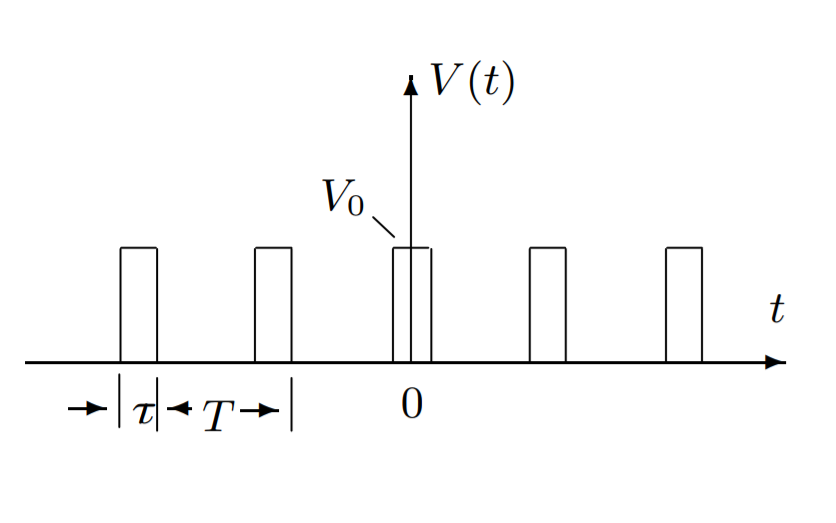
\includegraphics[width=0.9\linewidth]{sp1.png}}
				\caption{Прямоугольные импульсы}
			\end{minipage}
			\begin{minipage}[h]{0.5\linewidth}
				\center{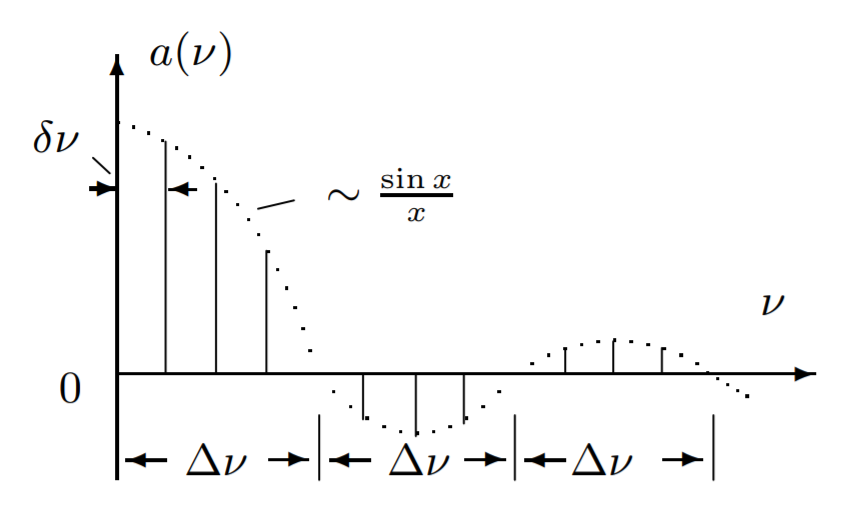
\includegraphics[width=0.9\linewidth]{sp2.png}}
				\caption{Спектр последовательности прямоугольных импульсов}
			\end{minipage}
		\end{figure}
	
	Назовем \textit{шириной спектра} $\Delta \omega$ расстояние от главного максимума ($\omega =0$) до первого нуля огибающей, возникающего при $n=\dfrac{2\pi}{\tau \Omega_{1}}$. При этом 

	$$\Delta \omega \tau \backsimeq 2 \pi $$
	
	 или 
	
\begin{equation}\label{neopr}
	\Delta \nu \Delta t \backsimeq 1
\end{equation}
		
	Полученное соотношение взаимной связи интервалов $\Delta \nu$ и $\Delta t$ является
	частным случаем соотношения неопределенности в квантовой механике.
	
	\item \textbf{Периодическая последовательность цугов} гармонического колебания $V_{0}\cos(\omega_{0}t)$ с длительностью цуга $\tau$ и периодом повторения $T$ (рис. 3).
	
	Функция $f(t)$ снова является четной относительно $t=0$. Коэффициент при $n$-й гармонике равен
	
	$$a_{n}=\dfrac{2}{T}\int\limits_{-\frac{\tau}{2}}^{\frac{\tau}{2}}V_{0}\cos(\omega_{0}t)\cos(n \Omega_{1} t)dt=V_{0}\dfrac{\tau}{T} \bigg(\dfrac{\sin[(\omega_{0}-n\Omega_{1})\frac{\tau}{2}]}{(\omega_{0}-n\Omega_{1})\frac{\tau}{2}}+\dfrac{\sin[(\omega_{0}+n\Omega_{1})\frac{\tau}{2}]}{(\omega_{0}+n\Omega_{1})\frac{\tau}{2}} \bigg)$$ 
	
	Зависимость для случая, когда $\frac{T}{\tau}$ равно целому числу, представлена на рис. 4. Сравнивая спектр последовательности прямоугольных импульсов и цугов мы видим, что они аналогичны, но их максимумы сдвинуты по частоте на величину $\omega_{0}$.
	
	\begin{figure}[h]
		\begin{minipage}[h]{0.5\linewidth}
			\center{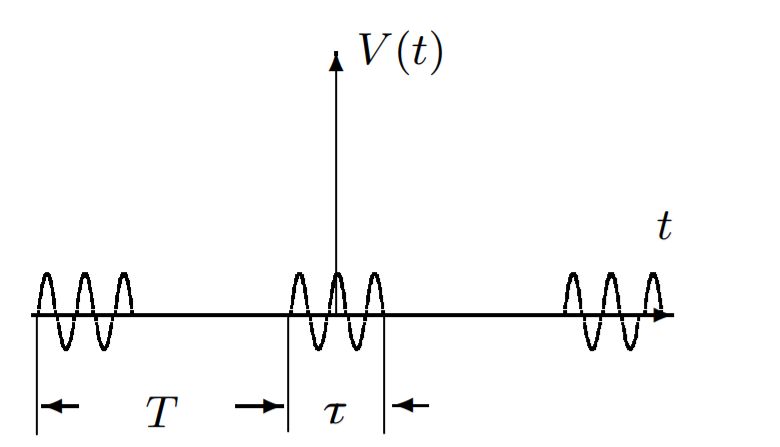
\includegraphics[width=0.9\linewidth]{sp3.png}}
		\end{minipage}
		\begin{minipage}[h]{0.5\linewidth}
			\center{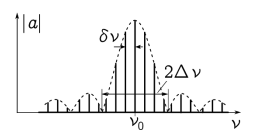
\includegraphics[width=0.9\linewidth]{sp4.png}}
			\caption{Спектр последовательности цугов}
		\end{minipage}
	\end{figure}

	\item \textbf{Амплитудно-модулированные колебания.} Рассмотрим гармонические колебания высокой частоты $\omega_{0}$ , амплитуда которых медленно меняется по гармоническому закону с частотой $\Omega$ ($\Omega \ll \omega_{0})$) (рис. 5):
	
	$$f(t)=A_{0}[1+m\cos\Omega t]\cos \omega_{0}t.$$
	
	Коэффициент $m$ называют \textbf{глубиной модуляции}. При $m<1$ амплитуда колебаний меняется от минимальной $A_{min}=A_{0}(1-m)$ до максимальной $A_{max}=A_{0}(1+m).$ Глубина модуляции может быть представлена в виде
	
\begin{equation}\label{m}
	 m=\dfrac{A_{max}-A_{min}}{A_{max}+A_{min}}
\end{equation}
	
	Простым тригонометрическим преобразованием можно найти спектр амплитудно - модулированных колебаний:
	\\
\begin{equation}\label{a}
	f(t)=A_{0}\cos(\omega_{0} t)+\dfrac{A_{0}m}{2}\cos(\omega_{0}+\Omega)t+\dfrac{A_{0}m}{2}\cos(\omega_{0}-\Omega)t.
\end{equation}
		
		\begin{figure}[h]
			\begin{minipage}[h]{0.5\linewidth}
				\center{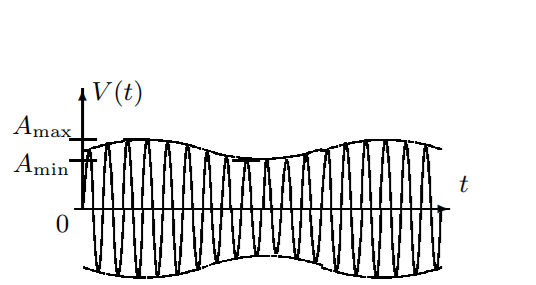
\includegraphics[width=0.9\linewidth]{sp5.png}}
				\caption{Модулированные гармонические колебания}
			\end{minipage}
			\begin{minipage}[h]{0.5\linewidth}
				\center{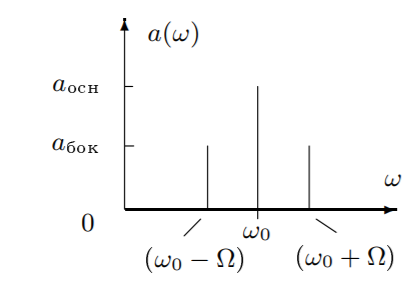
\includegraphics[width=0.9\linewidth]{sp6.png}}
				\caption{Спектр модулированных гармонических колебаний}
			\end{minipage}
		\end{figure}
		
		Спектр таких колебаний содержит три составляющих  основную
		компоненту и две боковых (рис. 6). Первое слагаемое в правой части представляет собой исходное немодулированное колебание
		с основной (несущей) частотой $\omega_{0}$ и амплитудой $a_{осн} = A_{0}$ . Второе и третье слагаемые соответствуют новым гармоническим колебаниям с частотами $\omega_{0} + \Omega$ и $\omega_{0} - \Omega$. Амплитуды этих двух колебаний одинаковы и составляют $\dfrac{m}{2}$ от амплитуды немодулированного колебания:
		$a_{бок} = \dfrac{A_{0}m}{2}$. Начальные фазы всех трех колебаний одинаковы.
	\end{enumerate}
\section*{Установка}

Установка, используемая в работе, представлена на рис. \ref{fig:scheme}.
\begin{figure}[h]
	\centering
	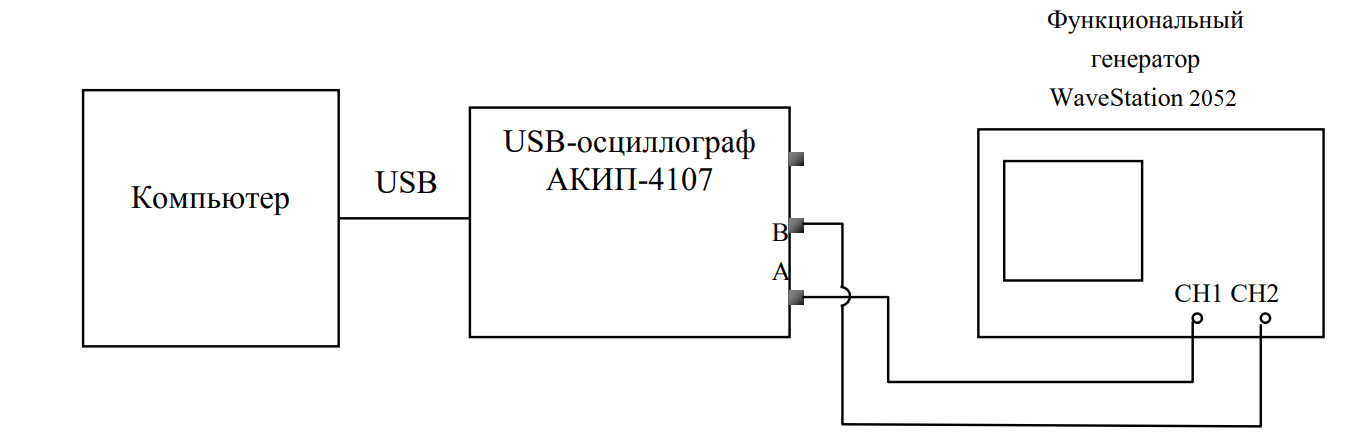
\includegraphics[width=1\linewidth]{sp9.png}
	\caption{Схема экспериментальной установки}
	\label{fig:scheme}
\end{figure}
Функциональный генератор позволяет сформировать два различных электрических сигнала, которые выводятся на два независимых канала USB-осциллографа.

Инструментальные погрешности считаются малыми.
\\
\textit{{Компьютер  с \emph{PicoScope 6}}} \\
\textit{Функциональный генератор \emph{waveStation 2052}} \\
\textit{USB-осциллограф \emph{АКИП-4108}} \\

\section*{Задание}

\indent \textbf{1) - 2)} Схема собрана и настроена в соответствие с лабником \\

\section*{А. Исследование спектра периодической последовательности 
прямоугольных импульсов и проверка соотношений неопределённостей}

\indent \textbf{3)} Выставляем на генераторе $\nu = \frac{1}{T} = 1$ кГц, $\tau = \frac{T}{20} = 50$ мкс.  

\begin{figure}[h]
    \centering
    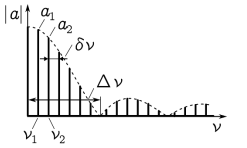
\includegraphics[width=0.3\linewidth]{sp10.png}
    \caption{Вводимые обозначения}
\end{figure}

\indent \textbf{4) - 6)} Получаем картинку вида: 

Получаем устойчивую картинку как на рис. 8. 

При увеличении $ \nu = \frac{1}{T} $ в 2 раза с постоянной $\tau$, ширина спектра - $\Delta \nu$ и $ \delta \nu $ - частота 1-й гармоники увеличивается во столько же раз. 

Заметим, что при уменьшении $ \tau $ вдвое при $\nu = const$, ширина спектра  - $\Delta \nu$ увеличивается в 2 раза и в 2 раза возрастает амплитуда спектра - $|a|$, в свою очередь $\delta \nu = const$.

\indent \textbf{7)} Фиксируем параметры $\nu = 1000$ Гц и $\tau = 50$ мс. И используя формулы: 
\begin{equation}
    \nu_n = \frac{n}{T}, \;\;\;\;\; |a_n| = \frac{|\sin(\frac{\pi n \tau}{T})|}{\pi n} = \frac{\tau}{T} \cdot \frac{|\sin (\pi \nu_n \tau)|}{\pi n \nu_n} 
\end{equation}

Заполняем табличку из методички для убеждения в верности теоретических выкладок:
\begin{tabular}{|l|r|r|r|r|r|r|r|r|}
\hline
$n$ & 1      & 2      & 3      & 4      & 5      & 6      & 7      & 8      \\ \hline
 $\nu_n^{\text{эксп}}$, Гц & 1016   & 2034   & 3019   & 3996   & 5018   & 5994   & 7009   & 7993   \\ \hline
 $\nu_n^{\text{теор}}$, Гц & 1000   & 2000   & 3000   & 4000   & 5000   & 6000   & 7000   & 8000   \\ \hline
 $|a_n^{\text{теор}}|$, усл. ед. & 0.0498 & 0.0492 & 0.0482 & 0.0468 & 0.0450 & 0.0429 & 0.0405 & 0.0378 \\ \hline
 $|a_n^{\text{эксп}}|$, мВ & 299.8  & 280.0  & 273.0  & 267.4  & 256.2  & 243.1  & 228.2  & 217.0  \\ \hline
 $|a_n^{\text{теор}}/a_1^{\text{теор}}|$ & 1      & 0.934  & 0.911  & 0.892  & 0.855  & 0.811  & 0.761  & 0.724  \\ \hline
 $|a_n^{\text{эксп}} / a_1^{\text{эксп}}|$ & 1      & 0.988  & 0.967  & 0.939  & 0.904  & 0.862  & 0.814  & 0.760  \\ \hline
 $\mathcal{E}_n,$ \% & 0 & 5.6    & 6.0    & 5.2    & 5.6    & 6.1    & 6.7    & 4.9    \\ \hline
\end{tabular} \\
Получаем отличие не более чем на 7\% что есть хороший результат.

\indent \textbf{8)} Фиксируем значение $\nu = 1$ кГц ($T = 1$ мс) и измерим зависимость ширины спектра $\Delta \nu$ от $\tau$, опорной гармоникой будем считать ту, у которой будет минимальная амплитуда ($|a_n| \rightarrow 0$).

\begin{tabular}{|l|r|r|r|r|r|r|r|r|}
\hline
$\tau$, мкс & 20    & 30    & 50    & 90    & 110  & 140  & 170  & 200  \\ \hline
$\Delta \nu,$ кГц & 48.83 & 33.05 & 20.03 & 10.98 & 8.98 & 7.04 & 5.99 & 5.02 \\ \hline
\end{tabular}

\indent \textbf{9)} Теперь снимем зависимость $\delta \nu$ от $T$, для этого фиксируем $\tau = 100$ мкс и изменяем $T$ в диапазоне от $2\tau$ до $50\tau$

\begin{tabular}{|l|r|r|r|r|r|r|r|r|}
\hline
$\nu$, кГц & 5   & 4   & 3   & 2   & 1    & 0.5  & 0.2  & 200                   \\ \hline
$T$, мкс & 200 & 250 & 333 & 500 & 1000 & 2000 & 5000 & 5.02                  \\ \hline
$\delta \nu$, кГц & 5   & 4   & 3   & 2   & 1    & 0.5  & 0.2  & \multicolumn{1}{l|}{} \\ \hline
\end{tabular}

\indent \textbf{10)} Построим требуемые графики:

\begin{minipage}{0.5\textwidth}
      \begin{tikzpicture}
        \begin{axis}[
          width=,
          height=,
          xlabel={$1/\tau,~\text{кГц}$},
          ylabel={$\Delta \nu,~\text{кГц}$},
          MyStyle1,
          ]
          \draw[blue, domain=0:100] plot (\x,0.975*\x-0);
          \addplot[purple, only marks] plot [error bars/.cd,
                x dir=both, x fixed = 0.05,
                y dir=both, y explicit,
                      ] table [
                      x=1/t, y=DeltaNu,
                x error minus=null, x error plus=null, y error minus=null, y error plus=null, col sep=comma] {DeltaNu(t^-1).csv};
        \end{axis}
      \end{tikzpicture}
    \end{minipage}
\begin{minipage}{0.5\textwidth}
      \begin{tikzpicture}
        \begin{axis}[
          width=,
          height=,
          xlabel={$\nu,~\text{кГц}$},
          ylabel={$\delta \nu,~\text{кГц}$},
          MyStyle1,
          ]
          \draw[blue, domain=0:100] plot (\x,1*\x-0);
          \addplot[purple, only marks] plot [error bars/.cd,
                x dir=both, x fixed = 0.05,
                y dir=both, y explicit,
                      ] table [
                      x=Nu, y=deltaNu,
                x error minus=null, x error plus=null, y error minus=null, y error plus=null, col sep=comma] {DeltaNu(t^-1).csv};
        \end{axis}
      \end{tikzpicture}
    \end{minipage}
    \\
    из графиков получается что $$\Delta \nu \cdot \tau \approx 1$$ $$\delta \nu \cdot T \approx 1 $$
    Что прекрасно соответствует теории.

\section*{Б. Наблюдение спектра периодической последовательности цугов}
\indent \textbf{11) - 12)} По методичке выставляем следующие параметры цугов на генераторе:
\begin{itemize}
    \item $\nu_0 = 50$, кГц
    \item $\tau = 1$, мс
    \item $N = 5$
\end{itemize}
Получаем устойчивую картину как на рис 3.

\indent \textbf{13)} 
\begin{itemize}
    \item меняем $\tau$: при увеличении в n раза $\tau$ уменьшается $\delta \nu$ в n раз, при уменьшении аналогично,
    \item меняем $N$: при уменьшении в n раз $N$ увеличивается $\delta \nu$ в n раз и $|a|$ уменьшается в n раз, при увеличении аналогично,
    \item меняем $\nu_0$: уменьшая $\nu_0$ увеличивается $\Delta \nu$ и $|a|$, а $\delta \nu$ не меняется.
\end{itemize}
\indent \textbf{14)}  Выберем 2 набора величин и посмотрим на отличия:\\
$\tau_1 = 5$, мс, $\tau_2 = 5$, мс; \\
$N_1 = 10$, $N_2 = 10$, мс; \\
$\nu_0_1 = 30$, кГц, $\nu_0_2 = 40$, кГц; $\Rightarrow$\\
$\Delta \nu_1 = 3$, кГц, $\Delta \nu_2 = 4$, кГц
$\Delta \text{центра} = 10$, кГц $\Rightarrow$ теорема смещения верна.

\section*{Г. Исследование спектра амплитудно-модулированного сигнала}
\indent \textbf{19)-20)} Выставляем режим модуляции по амплитуда со следующими параметрами: \\
$\nu_0 = 50$, кГц \\
50\%, $m = 0.5$ \\
$\nu_{\text{мод}} = 2$, кГц \\
Проверим для них выполнение соотношения:
$$m = \frac{A_{max} - A_{min}}{A_{max} + A_{min}}$$
В нашем случае: $A_{max} =  1504,$ мВ, а $A_{min} = 506.3,$ мВ $\Rightarrow m = 0.497 \approx 0.5$

\indent \textbf{21)} Получили картину один в один как на правой картинке ниже.
\begin{figure}[h]
    \centering
    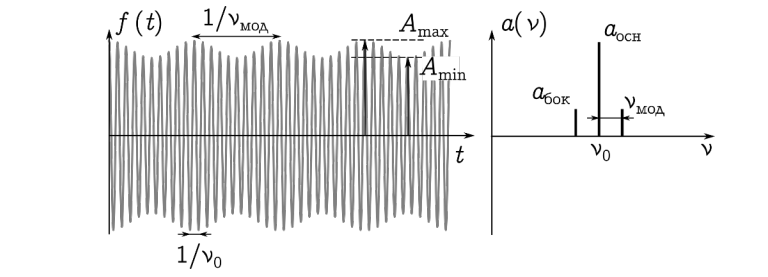
\includegraphics[width=0.75\linewidth]{zug.png}
    \caption{Вид спектра цуга}
\end{figure} \\
Где $\nu_{\text{центра}} = \nu_0 = 50$, кГц; $\nu_{\text{бок}}^1 = 48.12$, кГц; $\nu_{\text{бок}}^2 = 52.13$, кГц. Из чисел видно что $(\nu_{\text{бок}}^2 - \nu_{\text{бок}}^1) / 2 = \nu_{\text{мод}} = 2$, кГц.

\indent \textbf{22) - 23)} Снимем требуемые значения:
\begin{tabular}{|r|r|r|r|}
\hline
\multicolumn{1}{|l|}{$m_{\text{теор}}$, \%} & \multicolumn{1}{l|}{$|a_{\text{бок}}|$, мВ} & \multicolumn{1}{l|}{$|a_{\text{центр}}|$, мВ} & \multicolumn{1}{l|}{$\frac{a_{\text{бок}}}{a_{\text{центр}}}$}\\ \hline
10                     & 37.03                 & 712.2                 & 5.2                   \\ \hline
20                     & 72.6                  & 712.2                 & 10.2                  \\ \hline
40                     & 142.4                 & 712.2                 & 20.0                  \\ \hline
60                     & 212.2                 & 712.2                 & 29.8                  \\ \hline
70                     & 249.3                 & 712.2                 & 35.0                  \\ \hline
80                     & 286.3                 & 712.2                 & 40.2                  \\ \hline
90                     & 320.5                 & 712.2                 & 45.0                  \\ \hline
100                    & 359.7                 & 712.2                 & 50.5                  \\ \hline
\end{tabular}\\
Построим график:
\begin{minipage}{0.5\textwidth}
      \begin{tikzpicture}
        \begin{axis}[
          width=,
          height=,
          xlabel={$m\,~,\%$},
          ylabel={$\frac{a_{\text{бок}}}{a_{\text{центр}}}$},
          MyStyle1,
          ]
          \draw[blue, domain=0:100] plot (\x,0.500951585976628*\x-0.056594323873099484);
          \addplot[purple, only marks] plot [error bars/.cd,
                x dir=both, x fixed = 0.05,
                y dir=both, y explicit,
                      ] table [
                      x=m1, y=m2,
                x error minus=null, x error plus=null, y error minus=null, y error plus=null, col sep=comma] {m.csv};
        \end{axis}
      \end{tikzpicture}
    \end{minipage}
    Линейность графика и значение $k = (0.500\pm0.002)$ угла наклона прекрасно сводятся с теоретической точкой зрения.

\section*{Вывод}
Нами были изучены спектральные разложения различных периодических сигналов, а именно прямоугольные импульсы и цуги. Мы получили результаты хорошо сводящиеся с теорией, а именно взаимодействие $\delta \nu, \Delta \nu, \tau, T$ и т.д. друг с другом при их изменении, также проверили соотношение неопределенности $\delta \nu \cdot T \approx 1 $ и теорему о смещении.

Также нами была изучена амплитудная модуляция и проверено соотношение $\frac{a_{\text{бок}}}{a_{\text{центр}}} = \frac{m}{2}$
\end{document}